\documentclass[10pt,a4paper]{article}
\usepackage[utf8]{inputenc}
\usepackage{amsmath}
\usepackage{amsfonts}
\usepackage{amssymb}
\usepackage{graphicx}
\usepackage{float}
\usepackage[hidelinks]{hyperref}
\usepackage[left=1in,right=1in,top=1in,bottom=1in]{geometry}

\title{RISC-V RV32I UART Debugger Protocol}
\author{Trevor McKay}
\date{August 2020}
\graphicspath{{./figures/}}

\begin{document}

\maketitle
\tableofcontents

\newpage

\section{Overview}

This protocol aims to make hardware add-ons and software for your MCU easier to develop. Control flow operations
allow for easy manipulation of the state of the CPU as well as many low-level operations such
as memory and register editing, pause, or resume. Fortunately, all debugging operations can be
implemented with commands or a series of commands added by implementing this
protocol.

\medskip
\noindent\underline{\href{https://github.com/trmckay/riscv-uart-debugger}{Code repository}}

\section{Connections}

\begin{figure}[H]
    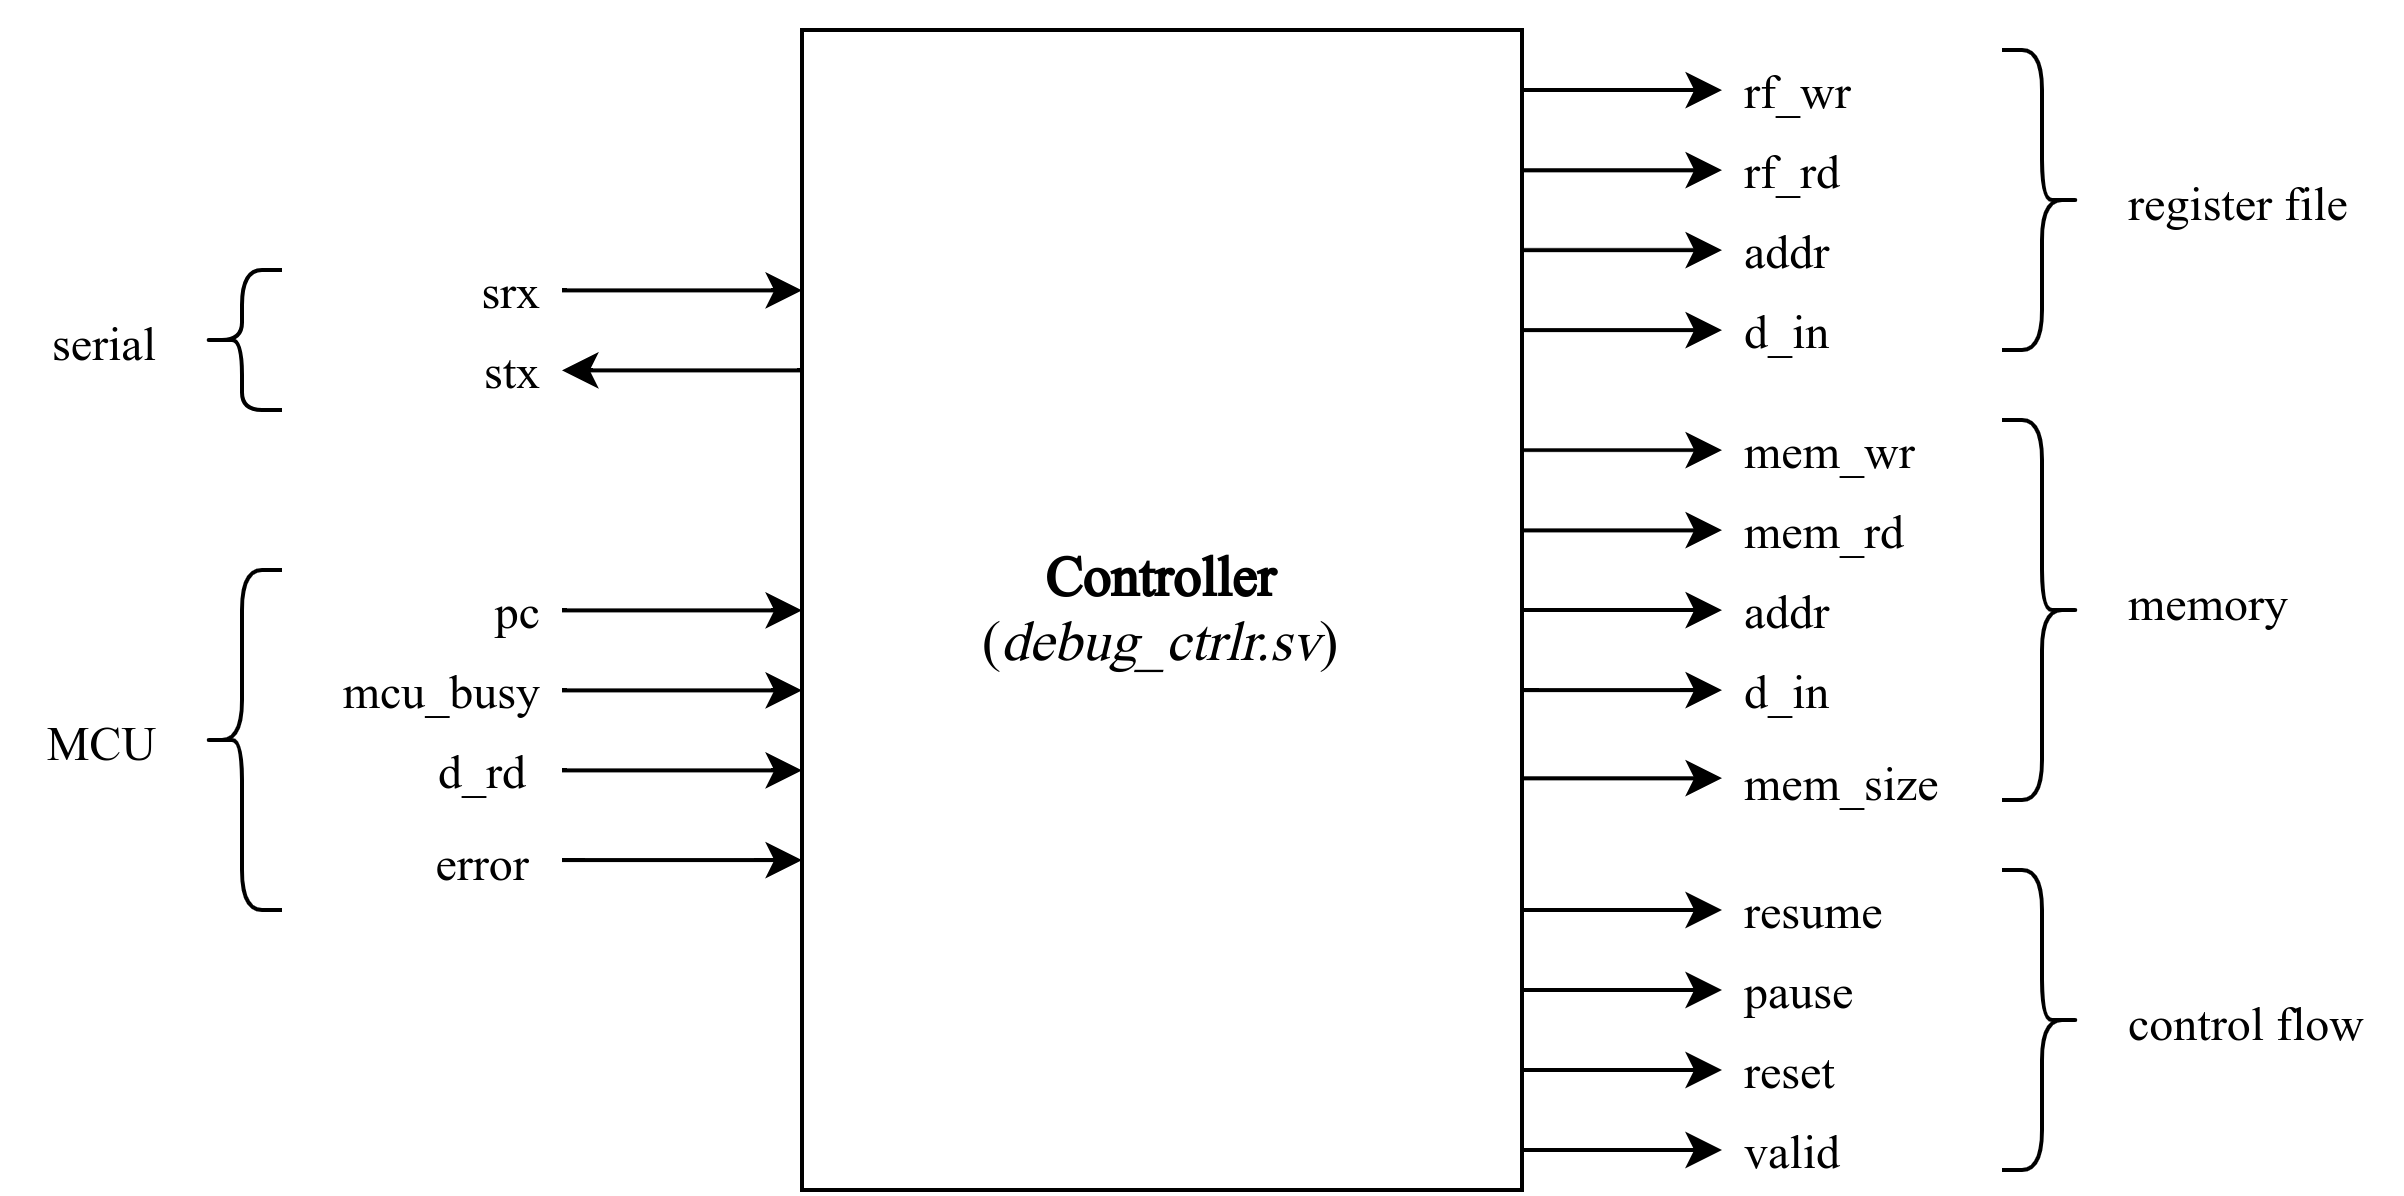
\includegraphics[width=\textwidth]{blackbox}
\end{figure}
\medskip

The module connects to the MCU, register file, and memory. Commands are recieved via serial
and decoded within the module. The signals \emph{rf\_wr}, \emph{rf\_rd}, \emph{addr}, and
\emph{d\_in} connect to the register file for reads and writes. The \emph{mem\_wr},
\emph{mem\_rd}, \emph{mem\_size}, \emph{addr}, and \emph{d\_in} connect to the memory
for reads and writes. Additionally, \emph{resume}, \emph{pause}, and \emph{reset} control
the flow of the MCU\@. Finally, the \emph{valid} signal determines wether or not the controller
is issuing a command.

\newpage
\section{Protocol}

It can be assumed that reads, writes, and resumes will only be issued while the MCU is paused. It
can also be assumed that only one command will occur at any time. If any two commands are issued at the
same time, it may be helpful to set \emph{error} and perhaps even do some handling.

\begin{enumerate}

    \item\textbf{valid}\\
    Indicates that the debugger is issuing a command. The MCU should respond accordingly on the next
    positive clock edge. However, \emph{mcu\_busy} should be asserted immediately so that the
    controller goes into the waiting state on the next cycle. The \emph{valid} signal is one-shot;
    however, control signals such as \emph{pause} and \emph{resume} will be held until the MCU is
    finished.

    \item\textbf{resume}\\
    The MCU should resume normal operation. If this takes more than one cycle,
    keep \emph{mcu\_busy}high to indicate this.

    \item\textbf{pause}\\
    The MCU should appear to stop execution after the current instruction completes. The
    \emph{mcu\_busy} signal should be asserted as soon as \emph{pause} and \emph{valid} are both
    high. For multicycle MCUs, the MCU should not fetch any more instructions (this can be done by
    injecting no-ops) once the pause begins. Only when the current instruction has committed
    all of its changes should \emph{mcu\_busy} go low. Pipelined MCUs will also need to halt
    instruction fetching, but will additionally need to flush the pipeline of all partially completed
    instructions. Once again, \emph{mcu\_busy} should only go low once the flush is completed.
    The currrent program count should be fed into the \emph{d\_rd} port to inform the client of the
    current point of execution.

        \begin{verbatim}
                 clk:  __|¯¯|__|¯¯|__|¯¯|__|¯¯|__|¯¯|__|¯¯

            mcu_busy:  ______________|¯¯¯¯¯¯¯¯¯¯¯|_________

               pause:  ______________|¯¯¯¯¯¯¯¯¯¯¯|_________

               valid:  ______________|¯|___________________
        \end{verbatim}

    \item\textbf{reset}\\
    The program counter should be set to zero. It is worth noting that this only resets the point of
    execution, not the contents of memory.

    \item\textbf{mem\_rd}\\
    The MCU should read the memory at \emph{addr}. The \emph{mcu\_busy} should go
     high at or before the next positive clock edge until the memory read is complete. The
    controller will attempt to read the data \emph{d\_rd} on the first positive clock edge that
    \emph{mcu\_busy} is low. If the address is out of range, set \emph{error} to high.

        \begin{verbatim}
                 clk:  __|¯¯|__|¯¯|__|¯¯|__|¯¯|__|¯¯|__|¯¯

            mcu_busy:  ________|¯¯¯¯¯¯¯¯¯¯¯¯¯¯|___________

                d_rd:  <______ Z ____________><__ 0x17 __>

              mem_rd:  ________|¯¯¯¯¯¯¯¯¯¯¯¯¯¯|___________

               valid:  ________|¯|________________________
        \end{verbatim}

    \newpage
    \item\textbf{mem\_wr}\\
    The MCU should write the data \emph{d\_in} to the memory at \emph{addr}. The \emph{mcu\_busy}
    should go high at or before the next positive clock edge until the memory write is complete.

        \begin{verbatim}
                 clk:  __|¯¯|__|¯¯|__|¯¯|__|¯¯|__|¯¯|__|¯¯

            mcu_busy:  ______________|¯¯¯¯¯¯¯¯¯¯¯|________

                d_in:  <_________ 0x17 __________><_ Z __>

              mem_wr:  ______________|¯¯¯¯¯¯¯¯¯¯¯|________

               valid:  ______________|¯|__________________
        \end{verbatim}

    \item\textbf{rf\_rd}\\
    The MCU should read the register file at \emph{addr}. The \emph{mcu\_busy} signal should go
    high at or before the next positive clock edge until the read is complete. However, it is
    likely that the register file supports asynchronous reads. If this is the case, and the data
    will be ready on the following clock edge, \emph{mcu\_busy} does not need to be asserted.

        \begin{verbatim}
                 clk:  __|¯¯|__|¯¯|__|¯¯|__|¯¯|__|¯¯|__|¯¯

            mcu_busy:  ___________________________________

                d_rd:  <_____ Z ____><______ 0x17 _______>

              reg_rd:  _________|¯¯¯¯|____________________

               valid:  _________|¯|_______________________
        \end{verbatim}

    \item\textbf{rf\_wr}\\
    The MCU should write the data \emph{d\_in} to the memory at \emph{addr}. The \emph{mcu\_busy}
    should go high at or before the next positive clock edge until the memory write is complete.
    This should only take one cycle for the register file; if so, \emph{mcu\_busy} will not need to
    be asserted.

        \begin{verbatim}
                 clk:  __|¯¯|__|¯¯|__|¯¯|__|¯¯|__|¯¯|__|¯¯

                  pc:  <_____________ 0x0C ______________>

            mcu_busy:  ___________________________________

                d_in:  <________ 0x17 _____><_____ Z ____>

              reg_wr:  ______________|¯¯¯¯¯¯|______________

               valid:  ______________|¯|___________________
        \end{verbatim}

\end{enumerate}

\newpage
\section{Implementation suggestions}
There is no right or wrong way to implement this protocol, as long as the MCU responds correctly.
However, there are some ways to make this easier.

Firstly, give your MCU the ability to flush outside of just the \emph{pause} signal.
In other words, have a \emph{flush} signal internal to the MCU that can be activated at any time.
Not only does it better decompose the control operations, but it can be useful to have this
for interrupts.

Additionally, have a register or logic variable in the MCU to keep track of whether the pipeline
is performing an operation. Quickly being able to determine this by looking at a single variable
will make it easier to MUX between the MCU's internal inputs and the controller's inputs for
the memory and register file. The controller will hold signals except for \emph{valid}, so it is not
necessary to keep track of the type of operation.

\vspace*{\fill}
\begin{center}
    \noindent Contact Trevor McKay with questions.\\
    \href{mailto:trs.mckay@gmail.com}{trs.mckay@gmail.com}
\end{center}

\end{document}
